We used micro-benchmarks to test the performance of RVM commits and RVM
recovery. To test commits, we allocated a number of pages, made modifications
to each one of them, and measured the time it took for \verb|rvm_txn_commit()|
to complete. To test recovery, we first allocate a number of pages and
close the connection to the server. We then restart the connection using the
recovery flag and time how long it takes \verb|rvm_cfg_create()| to complete.
When benchmarking the IB backend, we run three trials for each number of pages,
restarting the server after each trial.

\subsection{IB Backend}
Figure \ref{fig:ib-commit-ubm} shows the results of the commit micro-benchmark
using the IB backend. At the smallest page count, the commit time is around
150 microseconds. At 10K pages, the commit time has increased to 140 milliseconds.
As can be seen in the graph, the relation between page count and commit time
is fairly linear, with a slope of about 13.7 microseconds per page.
From examining the performance of \verb|rvm_txn_commit()| using the profiler,
we find that commit time is taken up mostly by sending the MULTI\_TXN\_CP
commands to the server, as well as performing RDMA writes to the remote memory pool.
Since these the number of commands and writes that need to be done scales
linearly with the number of pages, this accounts for the linear increase.

\begin{figure}[t!]
    \caption{IB Commit Micro-Benchmark Results}
    \includegraphics[width=\linewidth]{graphs/commit-results-rm.pdf}
    \label{fig:ib-commit-ubm}
\end{figure}

Figure \ref{fig:ib-recovery-ubm} shows the results of the recovery
micro-benchmark using the IB backend. Recovery is quite a bit slower than
commit. Recovering a single page takes about 50 milliseconds, while recovering
10,000 pages takes more than 2 seconds. The relationship between number of
pages and recovery time is also not entirely linear. The slope seems to
increase at about 5000 pages.

From profiling, we find that a large portion of time in recovery is spent
fetching the data for the recovered pages using RDMA reads. However, an even
larger portion of the time is spent registering pages with the Infiniband
driver. There is a potential optimization we could make here. A lot of the
pages being allocated are contiguous and so can be registered all at once.
Instead, we register each page one by one. Similarly, data for contiguous
pages could be fetched by a single RDMA read, instead of one read for each page.

We are uncertain what is causing the non-linear increase in recovery time.
It is possible that registering pages with the Infiniband driver takes
longer as the total number of pages registered grows larger.

\begin{figure}[t!]
    \caption{IB Recovery Micro-Benchmark Results}
    \includegraphics[width=\linewidth]{graphs/recovery-results-rm.pdf}
    \label{fig:ib-recovery-ubm}
\end{figure}

\subsection{RAMCloud Backend}
\begin{figure}[t!]
\begin{center}
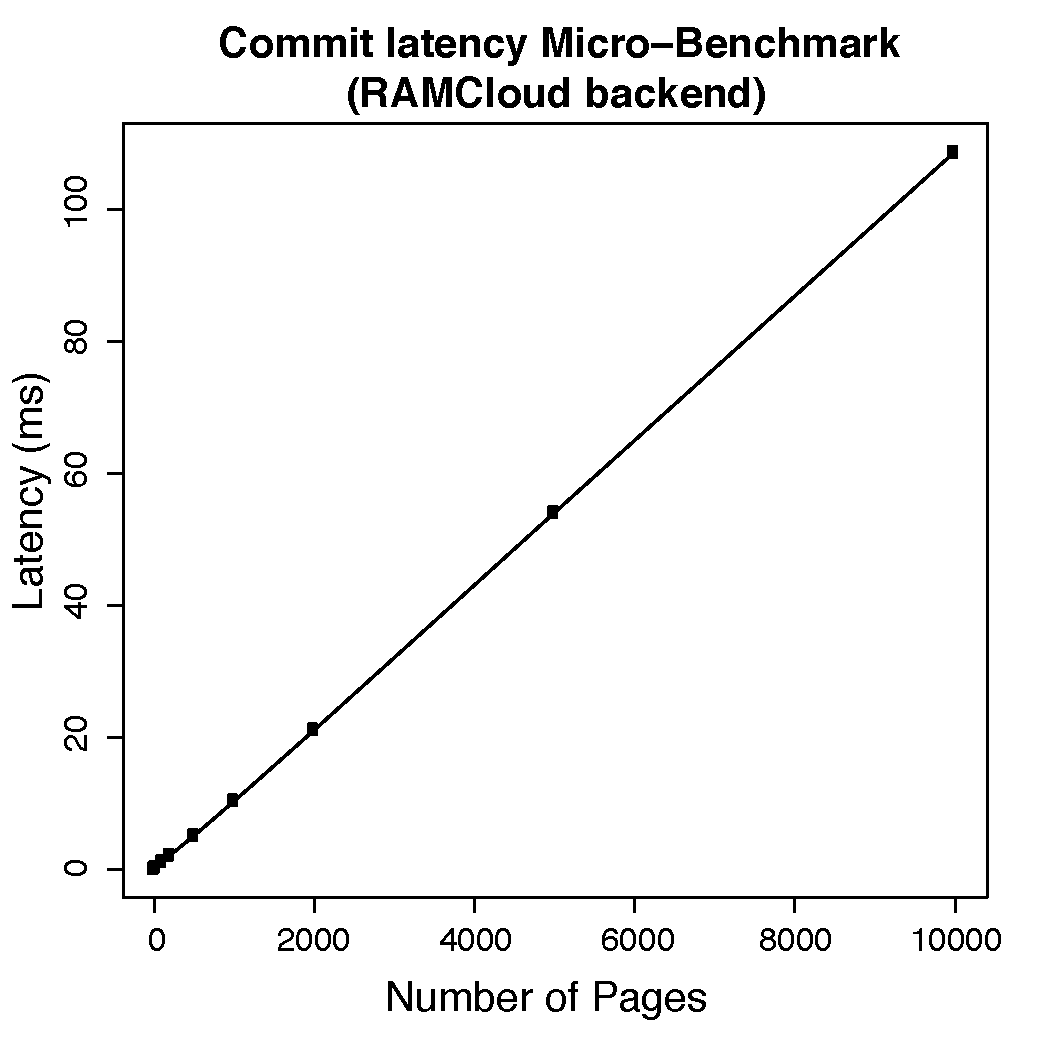
\includegraphics[scale=0.40]{graphs/commit_time_rc_latencies.pdf}
\end{center}
\caption{Commit time micro-benchmark when using the RAMCloud backend}
\label{fig:rc-commit-ubm}
\end{figure}

\begin{figure}[t!]
\begin{center}
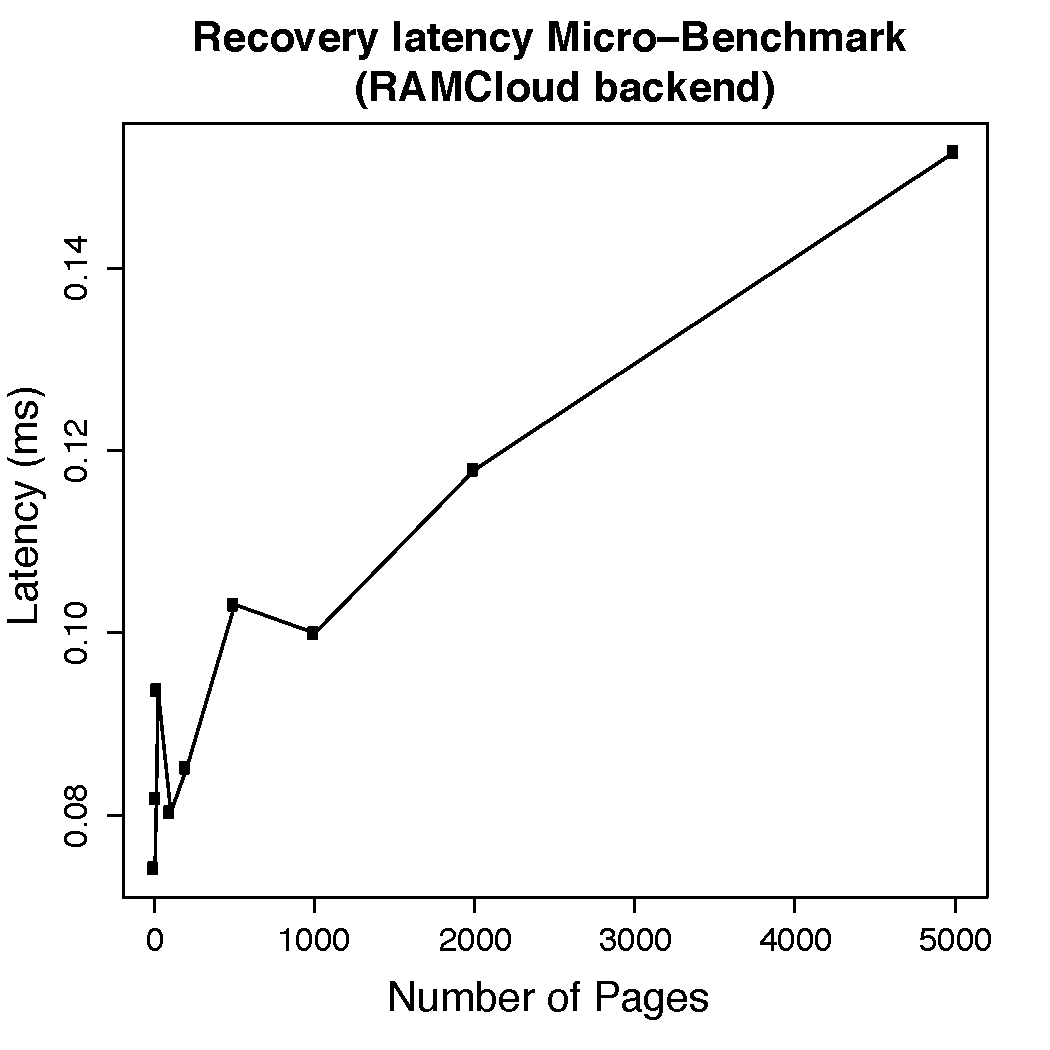
\includegraphics[scale=0.40]{graphs/recovery_time_rc_latencies.pdf}
\end{center}
\caption{Recovery time micro-benchmark when using the RAMCloud backend}
\label{fig:rc-recovery-ubm}
\end{figure}

Figure~\ref{fig:rc-commit-ubm} shows the results of the commit micro-benchmark when using the RAMCloud backend. 
The end-to-end latency of a commit operation is dominated by the number of pages to be committed, as each page write requires a round-trip to the RAMCloud server.
The RAMCloud backend also needs to save the table that contains the mapping between tags and keys in, but this only requires one interaction with the server.
The RAMCloud backend requires roughly 10 microseconds to write a page to RAMCloud. As can be seen in the graph, the commit time grows linearly with the number of pages as expected.

Figure~\ref{fig:rc-recovery-ubm} shows the results of the recovery micro-benchmark.
The end-to-end recovery time is mostly dominated by the time to establish a connection with the RAMCloud server (roughly 80ms).
Once the connection is established the RAMCloud backend retrieves the pages previously committed. The time to do this is dominated by the communication with the server, as in the commit benchmark, which grows linear with the number of pages.
Because of this we see a linear recovery time increase as the number of pages increases.
